%source: Farzaneh HW6-Q5


درشکل زیر، دیاگرام حالت یک مدار که دارای ورودی تک بیتی و خروجی دو بیتی است رسم شده است:

\begin{figure}[h]
	\centering
	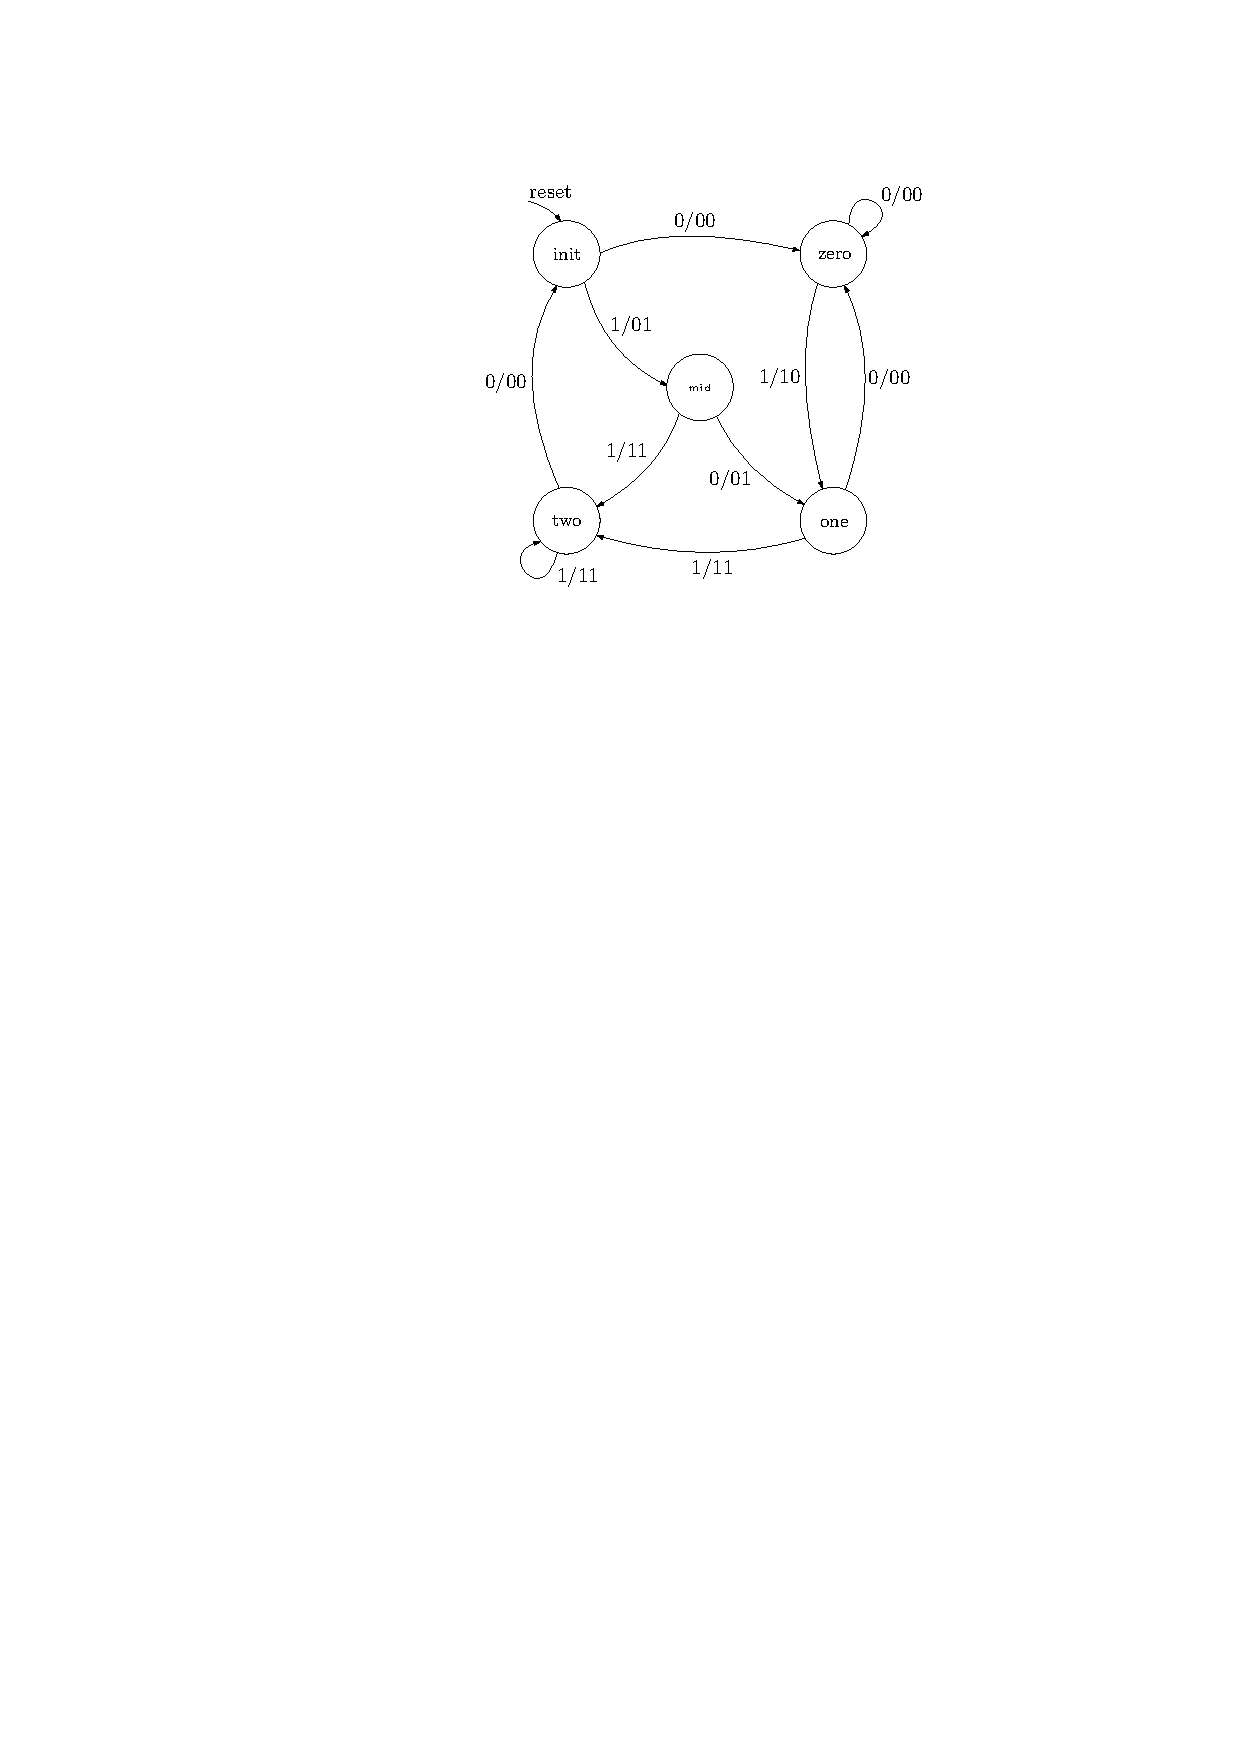
\includegraphics[width=0.4\textwidth]{fig/Q_basic8_.pdf}
	\label{fig:Q_basic_8}
\end{figure}



با درنظر گرفتن جدول زیر، جدول حالت این مدار را رسم کنید.

\begin{latin}
	\begin{table}[h!]
		\centering
		\begin{tabular}{|c|c|c|c|}
			\hline
			\textbf{State} & \multicolumn{3}{|c|}{\textbf{Encoding}} \\ \hline
			\textbf{Name} & $S_2$ & $S_1$ & $S_0$ \\ \hline
			init          & 1     & 1     & 1     \\ \hline
			mid           & 1     & 0     & 0     \\ \hline
			zero          & 0     & 0     & 0     \\ \hline
			one           & 0     & 0     & 1     \\ \hline
			two           & 0     & 1     & 0     \\ \hline
		\end{tabular}
	\end{table}
\end{latin}